\documentclass[a4paper]{article} 
\addtolength{\hoffset}{-2.25cm}
\addtolength{\textwidth}{4.5cm}
\addtolength{\voffset}{-3.25cm}
\addtolength{\textheight}{5cm}
\setlength{\parskip}{0pt}
\setlength{\parindent}{0in}

\usepackage[square,sort,comma,numbers]{natbib}
\usepackage{blindtext} % Package to generate dummy text
\usepackage{charter} % Use the Charter font
\usepackage[utf8]{inputenc} % Use UTF-8 encoding
\usepackage{microtype} % Slightly tweak font spacing for aesthetics
\usepackage{amsthm, amsmath, amssymb} % Mathematical typesetting
\usepackage{float} % Improved interface for floating objects
\usepackage{hyperref} % For hyperlinks in the PDF
\usepackage{graphicx, multicol} % Enhanced support for graphics
\usepackage{xcolor} % Driver-independent color extensions
\usepackage{pseudocode} % Environment for specifying algorithms in a natural way
\usepackage[mmddyy]{datetime} % Uses YEAR-MONTH-DAY format for dates

\usepackage{fancyhdr} % Headers and footers
\pagestyle{fancy} % All pages have headers and footers
\fancyhead{}\renewcommand{\headrulewidth}{0pt} % Blank out the default header
\fancyfoot[L]{} % Custom footer text
\fancyfoot[C]{} % Custom footer text
\fancyfoot[R]{\thepage} % Custom footer text
\newcommand{\note}[1]{\marginpar{\scriptsize \textcolor{red}{#1}}} % Enables comments in red on margin

\DeclareMathOperator*{\argmin}{arg\,min}

%----------------------------------------------------------------------------------------

\newcommand{\yourname}{Balthazar Neveu}
\newcommand{\youremail}{balthazarneveu@gmail.com}
\newcommand{\assignmentnumber}{2}

\begin{document}

\fancyhead[C]{}
\hrule \medskip
\begin{minipage}{0.295\textwidth} 
\raggedright
\footnotesize
\yourname \hfill\\
\youremail
\end{minipage}
\begin{minipage}{0.4\textwidth} 
\centering 
\large 
Lab session \# \assignmentnumber\\ 
\normalsize 
ALTEGRAD 2023\\ 
\end{minipage}
\begin{minipage}{0.295\textwidth} 
\raggedleft
\today\hfill\\
\end{minipage}
\medskip\hrule 
\bigskip



\section*{Coding results}

\subsection*{Task 1}
\begin{verbatim}
{'total_edges': 25998,
 'total_nodes': 9877}
max number of edges 48772626
\end{verbatim}


\subsection*{Task 2}
\begin{verbatim}
Graph has 429 connected components
Largest connected component:
{'total_edges': 24827,
 'total_nodes': 8638}
8638 total_nodes represent 87.46% of the graph
24827 total_edges represent 95.50% of the graph
\end{verbatim}


\subsection*{Task 3}
\begin{verbatim}
{'degree_of_nodes': {'max': 65,
                     'mean': 5.264351523742027,
                     'median': 3.0,
                     'min': 1}}
\end{verbatim}


\subsection*{Task 4}
\begin{verbatim}
\end{verbatim}\begin{figure}[ht]
        \centering
        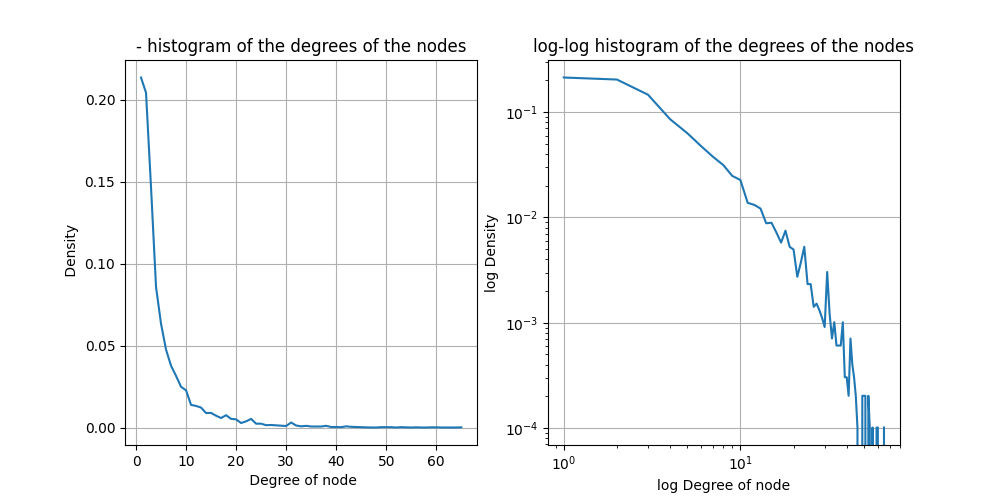
\includegraphics[width=.6\textwidth]{figures/histogram_degree_of_nodes.png}
        \caption{Histogram of degrees of the nodes}
\end{figure}
\begin{verbatim}
\end{verbatim}


\section{Question 1:}
Assume $G = (V, E)$ is an undirected graph of n nodes without self-loops. $|V|=n$.
\subsection*{Number of edges}
The maximum number of edges is the cardinal of the set of possible combinations of 2 nodes chosen from n nodes.
which is equal to the binomial coefficient $\binom{n}{2} = \frac{n!}{2! (n-2)!}$
\begin{equation}\label{eq 1.1}
|E| \leq \frac{n*(n-1)}{2}
\end{equation}
This can also be viewed when writing the adjacency matrix of a complete graph.
\begin{itemize}
    \item  A matrix full of 1 has $n^2$ elements
    \item set the diagonal to 0 to remove the self loops. $n*(n-1)$ elements
    \item Divide by two since we consider an undirected graph.
\end{itemize}


In the code the property is verified through an assert.

\subsection*{Number of triangles}
The maximum number of triangles is $\binom{n}{3} = \frac{n!}{3! * (n-3)!} = \frac{n*(n-1)(n-2)}{6}$ 
when choosing the combination of 3 nodes from n nodes.


\section{Question 2:}
%------------------------------------------------

\bibliographystyle{plain}
\bibliography{references}
\end{document}